\documentclass[11pt,a4paper]{article}
\usepackage{siunitx} % si eenheden
\usepackage{hyperref}					% maak PDF van de thesis navigeerbaar
\usepackage{url}
\usepackage[toc,acronym,xindy]{glossaries}%voor afkortingen
\usepackage{amsmath}
\usepackage[official]{eurosym} % om euro symbool te kunnen gebruiken
\usepackage{graphicx}
\usepackage{svg}
\usepackage[final]{pdfpages}
\usepackage[square,numbers]{natbib} 
\bibliographystyle{IEEEtran}
\usepackage{tabularx}  % betere tabellen
\usepackage[small,bf,hang]{caption} % verbetering captions
\captionsetup[table]{singlelinecheck=off} % caption van tabellen links uitlijnen


% =========== BELANGRIJK VR IN HET VERSLAG: Tonen dat je hebt nagedacht over dimensionering componenten! ===========

% MFA: zet zoekpad voor figure
\graphicspath{{fig/}}
\usepackage{float}                      % De optie H voor de plaatsing van figuren op de plaats waar je ze invoegt. bvb. \begin{figure}[H]

\begin{document}
\title{Embedded systems 2\\
	\Huge Report Cosy Cafeteria
}
\author{Robin Van de Poel\and Arthur Van den Storme\and Tobias Cromheecke\and Thomas Feys}
\date{\today}
\maketitle
\newpage

\tableofcontents
\newpage

\section{Intro}
To improve the experience of the students in the cafeteria, an embedded system will be developed to gather a variety of data. This data will then be display to the students through an online medium such as a website. The main focus will be to gather information about the amount of people that are in the cafeteria. There are two main goals. The first goal is to display the estimated waiting time to get a meal to the students. Secondly the amount of available seats will be tracked and displayed to the students. Next to this some additional information will be gathered. The temperature, air-quality and sound level will be monitored to give the student a general idea about the conditions in the cafeteria. This way the student can gauge if the cafeteria is suitable to study in at a certain moment. An overview of the envisioned system is displayed in figure~\ref{fig:system}. All the developed hardware and software is displayed at: \url{https://github.com/thomasf10/cosy_cafeteria}.
\begin{figure}[H]
	\centering
	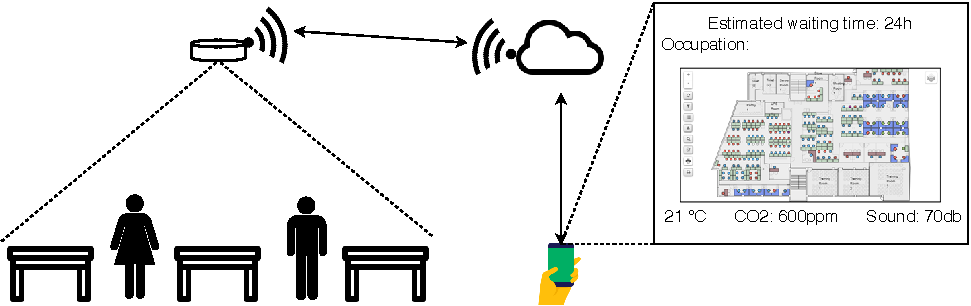
\includegraphics[width=1.0\linewidth]{situation.pdf}
	\caption{Situation sketch}
	\label{fig:system}
\end{figure}

\section{Specifications}
%Zoals we geleerd hebben in dit vak? eerst specs opstellen
%Hierbij moet de keuze's vermeld worden over:
% - Dimensions
% - Microcontroller 
\subsection{Functional specifications}
\begin{itemize}
	\item Monitor the available seats
	\item Monitor the queue to get a meal
	\item Display the data to the students
	\item Energy provision for 1 semester (4-5 months)
	\item Wireless coverage over the entire campus
	\item Measure new data every 10 minutes
	\item Send the data to the online medium every hour 
	\item If the data changes with a large amount (needs to be specified) update the online medium sooner
\end{itemize}

\subsection{Other technical specifications}
\begin{itemize}
	\item Enclosure: 10 x \SI{10}{\centi\meter}
	\item Easy deployment: the node must be easy to attach and detach from the sealing
	\item Must be easy to recharge (Wireless or via USB)
	\item Light weight: \SI{300}{\gram} (so it wont detach from the sealing)
\end{itemize}

\subsection{Non-technical specifications}
\begin{itemize}
	\item Cost: \euro{??}
	\item The data should be easy accessible to the students
\end{itemize}


\section{System architecture}
systeem wat uitleggen \dots
\textbf{!!EENS CHECKEN OF DE ARCHITECTUUR IN GROTE LIJNEN KLOPT}
An overview of the full system is displayed in figure~\ref{fig:architecture}.
\begin{figure}[H]
	\centering
	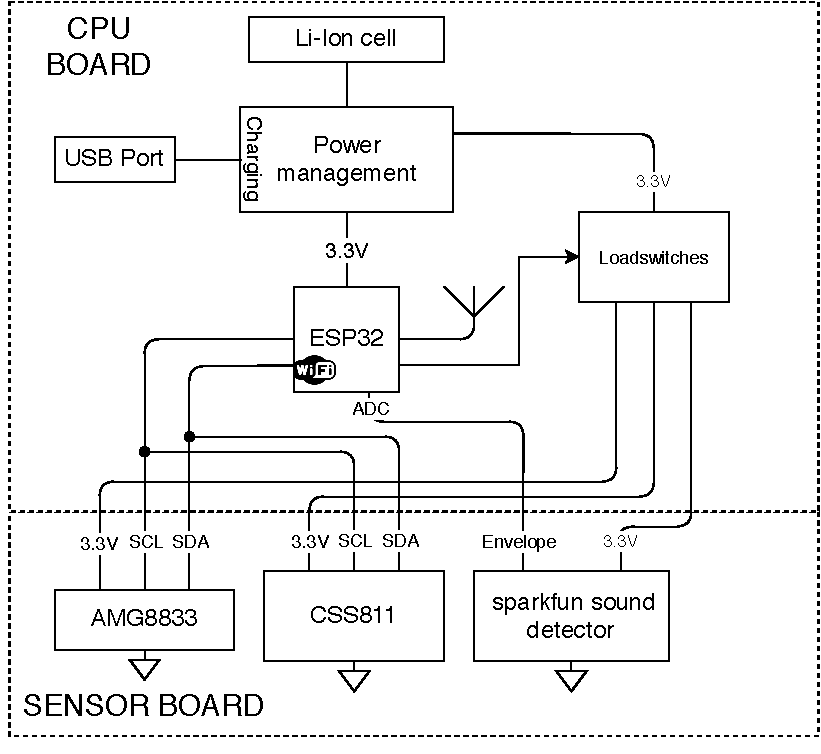
\includegraphics[width=1.0\linewidth]{architecture.pdf}
	\caption{System architecture}
	\label{fig:architecture}
\end{figure}
The developed system uses three sensors: 
\begin{itemize}
	\item AMG8833: IR grid sensor
	\item CSS811: air quality sensors
	\item Sparkfun sound detector: microphone
\end{itemize}
By incorporating these sensors in to the system, a variety of sensor data is gathered, namely: ambient temperature [\SI{}{\celsius}], $CO_2$-level [ppm], TVOC-level (total volatile organic compounds) [ppb] and sound level [db]. Next to this the AMG8833 captures the temperature af a two dimensional area in 8 by 8 pixels. 
\\ \\
The 'brain' of the system is an ESP32, this microcontroller has an integrated Wi-Fi module, which will be used to transmit the data. The gathered data is sent to a server, which stores the received data in a database. 
\\ \\
Alongside the reception of data from the ESP32, the server hosts a website which is used to display the data to the students. The website uses the pixel data to generate a heatmap of the cafeteria, this allows the students to see how many people are present in the cafeteria. Unfortunately one module cannot cover the entire cafeteria, to generate the heatmap. In order to do this, several modules have to be deployed in the cafeteria. In this project only one module will be constructed as a proof of concept. Next to the heatmap, the other sensor data is displayed on the website this includes: ambient temperature, $CO_2$-level, TVOC-level and the sound-level. Based on these parameters the students can gauge if the cafeteria is currently suitable as a study-location.


\section{Power management design}
This section explains the different trade-off's which were made in designing the power management part of the system. The first part in designing the power management is choosing a way to supply the circuit. In our case, the device needs to be deployed at the ceiling of a cafeteria. You can't just tap off the electricity cable at any point here, so our device will need a battery to supply the power. Our first aim was to supply the device as long as one semester. Another aspect was the ability to recharge the battery for environmental reasons. This excludes standard cell batteries that have a much lower energy density and are not rechargeable. Our choice was quickly made for the type of battery, namely a Lithium-Ion (Li-Ion) battery which will be discussed in section \ref{sec:liIon}.

\subsection{Lithium-Ion battery}\label{sec:liIon}
Lithium-Ion batteries are now a commonly used battery in consumer electronics. Li-Ion batteries is the most commonly used battery in phones, MP3 players and other portable equipment. The voltage of a single Li-Ion battery cell is usually fixed at 3.6 V or 3.7 V. We call this the nominal voltage. However, the actual voltage during use can vary from 2.4 V to 4.2 V. When the voltage drops below 2.4 V, the cell is discharged too deeply and damaged beyond repair. Therefore, a safety voltage of 3 V is often maintained. If the cell is discharged to this voltage, nothing is wrong. Charging a Li-Ion battery usually takes 3 hours. Don't be blinded by fast chargers for these batteries, practical tests have shown that it takes 3 hours until a battery is fully charged \cite{LiIon_ledscherp}. A few benefits of a Li-Ion battery are:
\begin{itemize}
	\item Very high energy density
	\item Minor self-discharge
	\item No memory effect
	\item High power, long service life
\end{itemize}
Some disadvantages are:
\begin{itemize}
	\item Relatively expensive to purchase
	\item Dangerous if used incorrectly, can explode/combust
	\item Need a protection circuit to not drop below the 2.4 V threshold value
	\item Charging and discharging process needed 
\end{itemize}
The most common Li-Ion battery is the 18650 cylindrical cell which is 18mm wide, 65mm long and the '0' stands for its cylindrical shape. Another common type of Lithium-Ion battery is the Lithium-Ion Polymer (Li-Po) battery.
%Li-Po's are:
%\begin{itemize}
%	\item Lighter
%	\item Faster recharge
%	\item Higher power: it's easy to produce batteries that can discharge 10C, 20C\footnote{\url{https://batteryuniversity.com/learn/article/what_is_the_c_rate}}.
%	\item Safer: less ability to explode/combust
%	\item Flexible: can bent (up to $90^\circ$) and deform + can be made in a variety of shapes
%	\item More expensive
%\end{itemize}
Li-Po's are preferred over standard Li-Ion batteries in application where weight reduction is important, fast charge opportunity is needed and which need a very high current during discharge time. Li-Po's are more used for drones (where lightweight is a requirement) and electric cars (fast charging requirement). Li-Po's are also less likely to combust or explode and are more expensive. Therefor a Li-Po would be overkill in our application \cite{LiIonVsLi-Po_Ovonic,LiIon_Wiki,Li-Po_Wiki}. 

\subsubsection{Selected battery}\label{sec:selected_battery}
The reason we chose a single cell Li-Ion battery was:
\begin{itemize}
	\item Voltage range: our microcontroller needs 3.3 V supply voltage, which is only a low dropout voltage of 0.4 V in comparison with the 3.7 V nominal voltage of a single cell Li-Ion battery. This results in less power dissipation in the voltage regulator. 
	\item Rechargeable: for environmental aspects
	\item High capacity: around 3000 mAh, to last a semester
\end{itemize}
The specifications of the chosen NCR18650B are:
\begin{itemize}
	\item Size/package: 18650
	\item Rated capacity: 3200 mAh
	\item Nominal voltage: 3.6 V
	\item Maximum voltage: 4.2 V
	\item Maximum charge current: 1625 mA
	\item Maximum discharge current: 6400 mA\footnote{Maximum discharge rate is 2C. This means discharging the battery capacity in 0.5 hours $\frac{3200 mAh}{0.5 h} = 6400 mA$ .} % https://batteryuniversity.com/learn/article/what_is_the_c_rate
	\item Maximum discharge voltage: 2.5 V
	\item Charge time: 4 hours
	\item No protection circuit
\end{itemize}
To charge the Li-Ion we had to include a charge circuit in our design. We found a high frequently used breakout board to charge a single cell Li-Ion battery via USB with battery protection \href{http://acoptex.com/project/9446/basics-project-082a-lithum-battery-charger-tp4056-at-acoptexcom/#sthash.3qJ5RSCy.AsMaJFMH.dpbs}{here}. Such a charge circuit would be perfect for our application. Due the reason we couldn't use a breakout board we had to integrate the components on one PCB. Unfortunately the components which were used on the breakout board were not available on the websites we're using to order components like Mouser, Digi-Key, Farnell, etc. After some research and a recommendation of a fellow student who had experience with battery charging applications in his master thesis, he advised to go for Texas Instruments IC's for charging Li-Ion batteries. The charger IC didn't had a protection circuit on it, so we also needed a circuit for this. Eventually we also went for a protection IC and voltage regulator of Texas Instruments. To protect the circuit for reverse polarity of the battery we also included an own-designed protection circuit which was first evaluated in LT Spice. All named components will be discussed in the following sections.

\subsection{Reverse polarity protection}
Reverse polarity protection is a nice feature to have te protect a circuit against polarity mismatches of the battery. For the design of this circuit we based us on a design found on the internet \href{http://kaktuscircuits.blogspot.com/2014/07/reverse-polarity-and-overvoltage.html}{here}. Before implementing this circuit in our design we first evaluated it's correct functioning using LT Spice in section \ref{sec:reverse_pol_prot_sim}.

\subsubsection{Simulation}\label{sec:reverse_pol_prot_sim}
Reverse polarity protection is simple done by including a P type MOSFET as shown in figure \ref{fig:reverse_polarity_protection_simulation}. Since the maximum voltage is limited to 4.2 V of the battery, there is no need for high drain-to-source voltage $V_{DS}$ requirements for the MOSFET. A suitable MOSFET was found \cite{bib:NTR2101P}. Normally there should be a zener diode placed between gate and source to protect the maximum gate-to-source voltage $V_{GS}$. Since the selected MOSFET's $V_{DS}$ = $V_{GS}$ = 8 V there is no need for a zener diode to clamp the voltage. 
% NTR2101P Spice model: https://www.digchip.com/application-notes/52/54566.php
\begin{figure}[H]
	\centering
	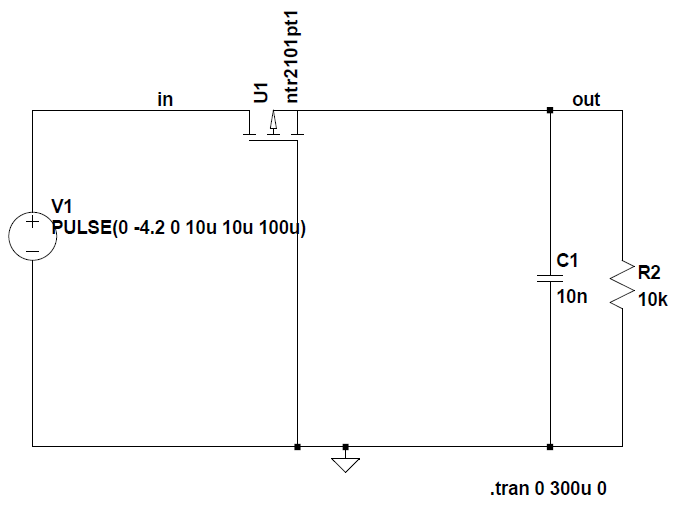
\includegraphics[width=0.8\linewidth]{reverse_polarity_protection_simulation.png}
	\caption{Simulation reverse polarity protection circuit}
	\label{fig:reverse_polarity_protection_simulation}
\end{figure}
Figure \ref{fig:Transient_response_negative_input_pulse} shows the transient response when applying a negative pulse at the input. As can be seen in the figure, the negative pulse doesn't come through the rest of the circuit. The voltage at the output is 0 V.
\begin{figure}[H]
	\centering
	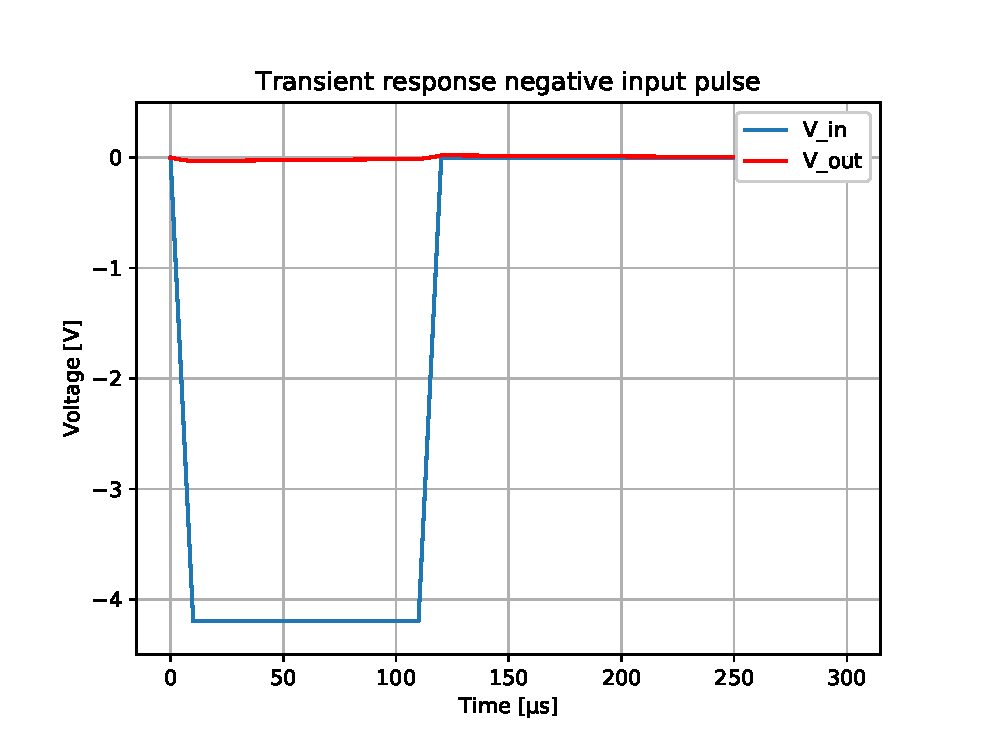
\includegraphics[width=0.8\linewidth]{Transient_response_negative_input_pulse.eps}
	\caption{Transient response negative input pulse}
	\label{fig:Transient_response_negative_input_pulse}
\end{figure}
When applying a positive pulse at the input, it can be seen in figure \ref{fig:Transient_response_positive_input_pulse} the output follows the input. We can evaluate the circuit works properly to protect against reverse polarity protection. Now it can be implemented in our design discussed in section \ref{fig:Transient_response_positive_input_pulse}.
\begin{figure}[H]
	\centering
	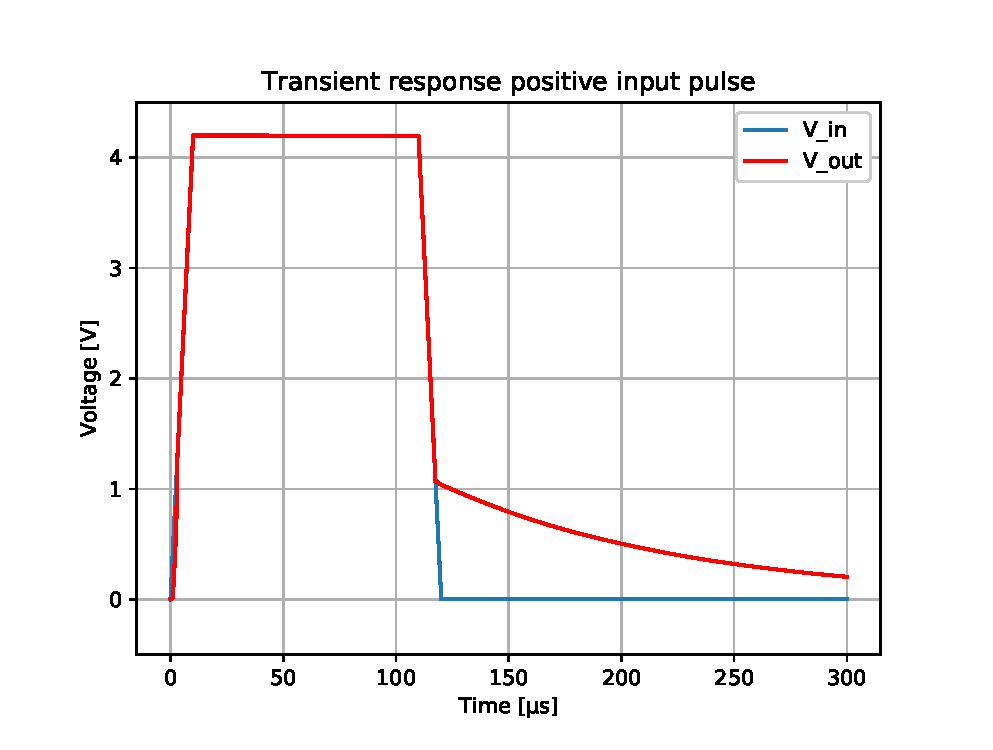
\includegraphics[width=0.8\linewidth]{Transient_response_positive_input_pulse.eps}
	\caption{Transient response positive input pulse}
	\label{fig:Transient_response_positive_input_pulse}
\end{figure}

\subsubsection{Implementation}\label{sec:reverse_pol_prot_implementation}
As a precaution we included two batteries in the first version of our design. This was done for debugging reasons: in case our real current consumption would be too high after trying every possibility to reduce it in software, we had an extra battery to meet our lifetime goal. It was possible to include an extra battery because the PCB dimensions were still lesser then 100 x 100 mm. JP1 is a footprint to solder a wire so we are able to measure the current using a current probe. When the battery is correct polarity of the battery is applied, +BATT is connected to VDD1.
\begin{figure}[H]
	\centering
	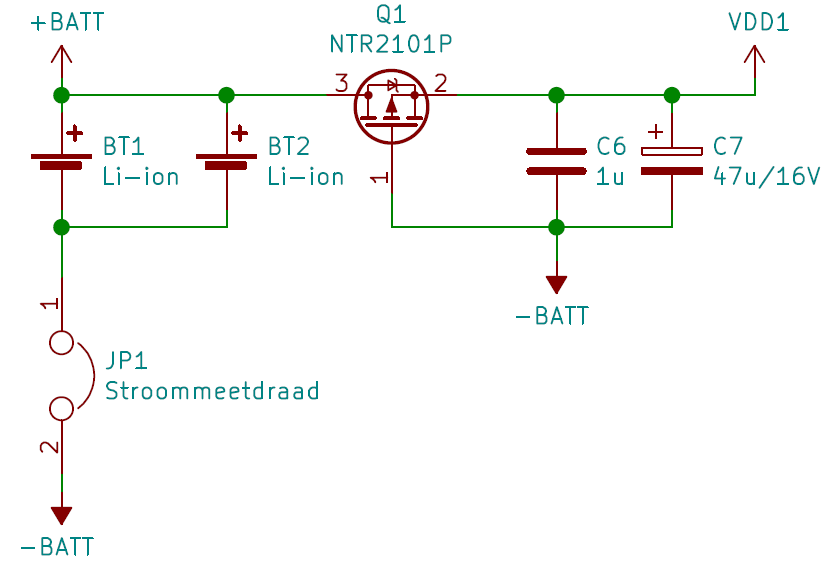
\includegraphics[width=0.8\linewidth]{reverse_polarity_protection.png}
	\caption{Reverse polarity protection circuit}
	\label{fig:reverse_polarity_protection}
\end{figure}

\subsection{Charging choice}
For charging you're free to choose at which voltage and current you charge. Eventually a Li-Ion charger IC will step down the voltage to the maximum 4.2 V for a cell. For charging you could design your own AC-DC converter, we went for the ability to charge the device using USB. Here for we rely on a power adapter which transforms 240 VAC to 5 VDC, or the ability to charge our device using a USB port on a computer. Figure \ref{fig:microUSBinput} shows the input connector micro USB type B with two decoupling capacitors $C_1$ and $C_2$. The charging voltage source is labeled as Vin.
\begin{figure}[H]
	\centering
	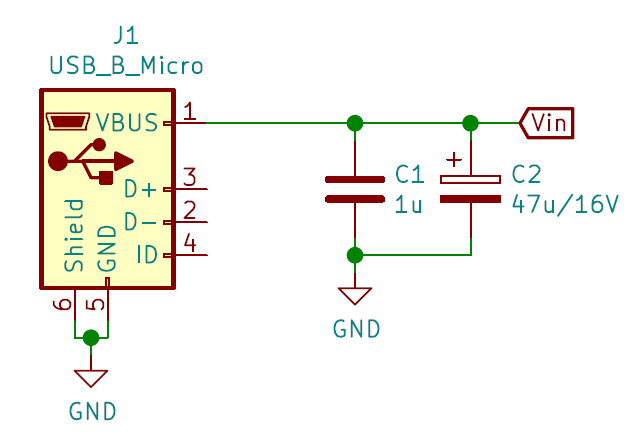
\includegraphics[width=0.8\linewidth]{microUSBinput.png}
	\caption{Micro USB type B input}
	\label{fig:microUSBinput}
\end{figure}

\subsection{Battery charging circuit}
We considerd many chips from different kind of manufacturers. As previously said a TP4056 IC charger is commonly used for single cell Li-Ion batteries, but it's not available on Digi-Key, Farnell, etc. Eventually we went with the BQ24075 IC from Texas Instruments. It's a great choice because it's made to charge a single cell Li-Ion battery, and it's perfectly fit to charge using a USB port. The IC operate from either a USB port or an AC adapter and support charge currents up to 1.5 A. The input voltage range with input overvoltage protection supports unregulated adapters. The USB input current limit accuracy and start up sequence allow the BQ24075 to meet USB-IF inrush current specifications\footnote{\url{http://www.testusb.com/inrush_issue.htm}}. Additionally, the input dynamic power management (VIN-DPM) prevents the charger from crashing incorrectly configured USB sources. An additional specification that was decisive in the choice of charger IC was the availability of 2 pins for status indication:
\begin{enumerate}
	\item \textbf{power good indication:} if the input voltage Vin is in specified range.
	\item \textbf{charge indication:} if the charger is charging (bright up LED) and when the charge cycle is complete (quench LED)
\end{enumerate}
Figure \ref{fig:bq24075_toegepast} shows the BQ24075 IC implemented in our design. A green LED D1 indicates the power good signal, and blue LED D2 indicates the charging stage. When no voltage is applied at the input Vin, the internal transistor Q1 is opened and Q2 is closed. Therefor VDD1 is connected to VDD2. During charge cycle both transistors Q1 and Q2 are closed allowing the battery to charge. The BQ24075 feature a SYSOFF input that allows the user to turn Q2 off and disconnect the battery from the OUT pin. This is useful for disconnecting the system load from the battery, factory programming where the battery is not installed or for host side impedance track fuel gauging, where the battery open circuit voltage level must be detected before the battery charges or discharges. We don't use this feature so we connect SYSOFF to GND to close Q2 for normal operating mode \cite{bib:BQ24075}. %Connect SYSOFF high to turn off the FET connecting the battery to the system output. When an adapter is connected, charging is also disabled. Connect SYSOFF low for normal operation. SYSOFF is internally pulled up to VBAT through a large resistor (approximately 5 M$\Omega$). Do not leave SYSOFF unconnected to ensure proper operation.
The other features of BQ24075 and schematic components will be discussed in sections \ref{sec:charging_phases} to \ref{sec:BQ24075_caps}.
\begin{figure}[H]
	\centering
	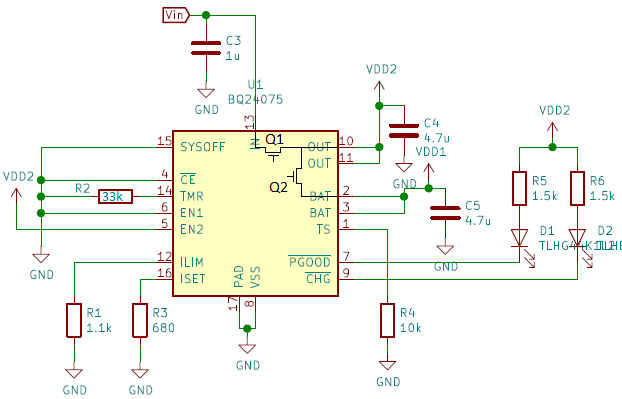
\includegraphics[width=0.9\linewidth]{bq24075_toegepast.png}
	\caption{Typical application circuit BQ24075}
	\label{fig:bq24075_toegepast}
\end{figure}

\subsubsection{Charging phases}\label{sec:charging_phases}
Set $\overline{CE}$ low to initiate battery charging. The battery is charged in three phases: 
\begin{enumerate}
	\item Conditioning pre-charge
	\item Constant current (CC) fast charge (current regulation) 
	\item Constant voltage (CV) tapering (voltage regulation)
\end{enumerate}
Figure \ref{fig:Charge _cycle} illustrates the three charging phases. In the pre-charge phase, the battery is charged at with the pre-charge current $I_{PRECHG}$. Once the battery voltage crosses the $V_{LOWV}$ threshold, the battery is charged with the fast-charge current $I_{CHG}$. As the battery voltage reaches $V_{BAT(REG)}$, the battery is held at a constant voltage of $V_{BAT(REG)}$ and the charge current tapers off as the battery approaches full charge. When the battery current reaches $I_{TERM}$, the CHG pin indicates charging done by going high-impedance.
\begin{figure}[H]
	\centering
	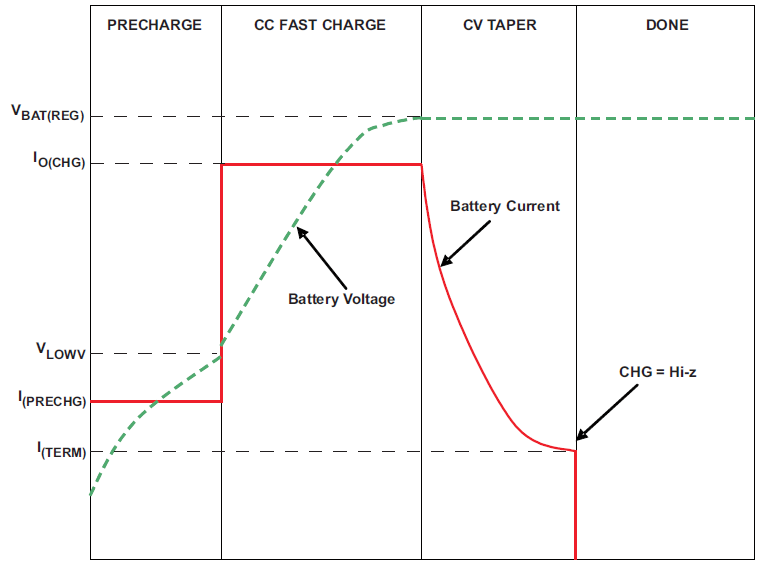
\includegraphics[width=1.0\linewidth]{Charge_cycle}
	\caption{Charge cycle \cite{bib:BQ24075}}
	\label{fig:Charge _cycle}
\end{figure}


\subsubsection{Set input current limit $I_{LIM}$}
The BQ24075 IC offers a fully compliant USB charger, meaning:
\begin{enumerate}
	\item Selectable 100 mA and 500 mA maximum input current
	\item 100 mA Maximum current limit ensures compliance to USB-IF standard
	\item Input-based dynamic power management (VINDPM) for protection against poor USB sources
\end{enumerate}
As shown in table \ref{table:USBmode}, EN1 and EN2 are used to configure the USB charge current.
\begin{table}[H]
	\caption{EN1/EN2 Settings \cite{bib:BQ24075}}
	\label{table:USBmode}
	\begin{tabular}{c|c|l}
		EN2 & EN1 & MAXIMUM INPUT CURRENT INTO IN PIN            				\\
		\hline
		0   & 0   & 100 mA. USB100 mode                          				\\
		0   & 1   & 500 mA. USB500 mode                          				\\
		1   & 0   & Set by an external resistor from ILIM to VSS (max. 1.5 A) 	\\
		1   & 1   & Standby (USB suspend mode)                  
	\end{tabular}
\end{table}
USB1.0 specifications allow devices to draw up to 500 mA from one port. USB operates at 5V, so that means a maximum of 2.5 watts. USB 2.0 has the same power limit. But later there were add-ons to the spec for battery charging, allowing up to 1.5A (7.5W) while data transfer is going on, and up to 5A if not. Few USB 2.0 devices can deliver that much power. Also note that the Micro USB connector is only rated to carry 2.1A (10.5W). USB 3.0 increases the power limit to 900mA (4.5W). The battery charging spec from USB 2.0 can optionally be supported \cite{USBpowers}. Since almost all USB chargers and ports are 2.0 and 3.0 nowadays, we can step up the current above 500 mA. The value of the input current limit $I_{LIM}$ is set by the resistor connected from the ILIM pin (pin 12) to VSS, and is given by \cite{bib:BQ24075}
\begin{equation}\label{equ:relationK_ILIM}
R_{ILIM} = \frac{K_{ILIM}}{I_{LIM}} \,,
\end{equation}
with 
\begin{equation}\label{equ:K_ILIM}
K_{ILIM} = 1610 A\Omega \,.
\end{equation}
The valid resistor range is 1.1 k$\Omega$ to 8 k$\Omega$. A value of 1.1 k$\Omega$ results in an input current limit 
\begin{equation}\label{equ:I_LIM}
I_{LIM} = \frac{1610 A\Omega}{1.1 k\Omega} = 1.46 A \,.
\end{equation}
The maximum input current limit 1.5 A is reached. \textbf{Caution:} make sure this current doesn't exceed the value of the maximum charge current of the battery, which is in our case within the permitted limit of 1625 mA (section \ref{sec:selected_battery}).


\subsubsection{Fast charge safety timer (TMR)}
TMR controls the pre-charge and fast-charge safety timers. Leave TMR open to set to default safety timers. Connect to VSS to disable safety timers. Connect a 18 k$\Omega$ to 72 k$\Omega$ resistor between TMR and VSS to program the timers a desired length. Reset the timers by toggling the CE pin, or by toggling EN1, EN2 pin to put the device in and out of USB suspend mode (EN1 = 1, EN2 = 1). The charge time of the battery is 4 hours (section \ref{sec:selected_battery}). We will calculate the TMR resistor $R_{TMR}$ to meet the desired charge time of 4 hours, using equation \cite{bib:BQ24075}
\begin{equation}
R_{TMR} = \frac{t_{MAXCHG}}{10 \cdot K_{TMR}} \,,
\end{equation}
with 
\begin{equation}
K_{TMR} = 48 \, s/k\Omega \,,
\end{equation}
\begin{equation}
t_{MAXCHG} = 4 hr \,.
\end{equation}
\begin{equation}
R_{TMR} = \frac{t_{MAXCHG}}{10 \cdot K_{TMR}} = \frac{4 \, hr \cdot 3600 \, s/hr}{10 \cdot 48 \, s/k\Omega} = 30 \, k\Omega
\end{equation}
Select a resistor value of 33 k$\Omega$, so it's E6-E12 compliant an to extend it charge time a little bit. Connect this resistor between TMR (pin 2) and VSS.


\subsubsection{Set fast charge current $I_{CHG}$}\label{sec:fastchargecurrent}
The value of fast-charge current $I_{CHG}$ is set by the resistor connected from the ISET pin to VSS, and is given by \cite{bib:BQ24075}
\begin{equation}\label{equ:relationK_ISET}
R_{ISET} = \frac{K_{ISET}}{I_{CHG}} \,,
\end{equation}
with
\begin{equation}\label{equ:K_ISET}
K_{ISET} = 890 A\Omega \,.
\end{equation}
The charge current limit is adjustable up to 1.5 A. The valid resistor range is 590 $\Omega$ to 8.9 k$\Omega$. If $I_{CHG}$ is programmed as greater than the input current limit $I_{LIM}$, the battery will charge at the rate of $I_{LIM}$ instead of $I_{CHG}$. In this case, the charger timers will be proportionately slowed down. The maximum charge current for the Panasonic NCR18650B battery is 1625 mA (section \ref{sec:selected_battery}). Set charge current to 1.3 A to have some margin for the battery lifetime and calculate the resistor value
\begin{equation}
R_{ISET} = \frac{890 A\Omega}{1.3 A} = 684.62 \Omega \approx 680 \Omega \,.
\end{equation}
Select the closest standard value (E6,E12,...), which for this case is 680 $\Omega$. Connect this resistor between ISET (pin 16) and VSS.
%The eventual charge current will be 
%\[ I_{CHG} = \frac{890 A\Omega}{680 \Omega} = 1.31 A \,. \]

%\subsubsection{Charge Current Translator}
%When the charger is enabled, internal circuits generate a current proportional to the charge current at the ISET input. The current out of $I_{SET}$ is 1/400 ($\pm$10\%) of the charge current. This current, when applied to the external charge current programming resistor, $R_{ISET}$, generates an analog voltage that can be monitored by an external host to calculate the current sourced from BAT.
%\[ V_{ISET} = \frac{I_{CHG}}{400} R_{ISET} \]


\subsubsection{TS function}
The TS-pin is the external NTC thermistor input. Connect the TS input to the NTC thermistor in the battery pack. TS monitors a 10 k$\Omega$ NTC thermistor. For applications that do not use the TS function, connect a 10 k$\Omega$ fixed resistor from TS to VSS to maintain a valid voltage level on TS.


\subsubsection{Selecting IN-, OUT-, and BAT-pin capacitors}\label{sec:BQ24075_caps}
In most applications, all that is needed is a high-frequency decoupling capacitor (ceramic) on the power pin, input, output and battery pins. Using the values shown on figure \ref{fig:bq24075_toegepast} (these are taken from the typical application circuit in \cite{bib:BQ24075}) is recommended. After evaluation of these voltage signals with real system operational conditions, one can determine if capacitance values can be adjusted toward the minimum recommended values (DC load application) or higher values for fast high amplitude pulsed load applications. Note if designed high input voltage sources (bad/wrong adaptors), the capacitor needs to be rated appropriately. Ceramic capacitors are tested to 2x their rated values so a 16-V capacitor may be adequate for a 30-V transient (verify tested rating with capacitor manufacturer).



\subsection{Battery protection circuit}\label{sec:bat_prot_circuit}
Due the battery we selected doesn't has an integrated protection circuit, we also needed to consider a battery protection circuit in our design. As discussed in section \ref{sec:liIon} it could lead to battery defect when the voltage of the battery drops below 2.4 V threshold value. A Li-Ion is also likely to explode/combust when charging too high in voltage or current. Therefor a protection circuit is always needed. We went for the BQ29700 which is a battery cell protection IC that provides an accurate monitor and trigger threshold for overcurrent protection during high discharge/charge current operation or battery overcharge conditions. The BQ29700 provides the protection functions for Li-Ion/Li-Po cells, and monitors across the external power FETs for protection due to high charge or discharge currents. Figure \ref{fig:bq29700_principeschema} shows a typical application circuit of the BQ29700 IC. In normal mode FETs Charge FET (CHG) and Discharge FET (DSG) are closed, however in one of the following conditions the FETs will open to stop the current flow from/to the battery:
%The system is operating in NORMAL mode when the battery voltage range is between the over-discharge detection threshold (VUVP) and the overcharge detection threshold (VOVP), and the V– pin voltage is within the range for charge overcurrent threshold (VOCC) to over-discharge current threshold (VOCD) when measured with respect to VSS. If these conditions are satisfied, the device turns ON the drive for COUT and DOUT FET control.
\begin{enumerate}
	\item \textbf{Overcharge detection (OVP):} When the cell exceeds the overcharge detection threshold voltage $V_{OVP}$ during charge, the safety circuit will interrupt the flow of current into the cell.% by opening CHG.
	When the overcharge voltage is exceeded, a delay of up to $t_{OVP}$ will occur before the FETs open the circuit.
	\item \textbf{Over-discharge detection (UVP):} When the cell exceeds the over-discharge detection threshold voltage $V_{UVP}$ during discharge, the safety circuit will interrupt the flow of current out of the cell.% by opening DSG. 
	When the over-discharge voltage is reached, a delay $t_{UVP}$ will occur before the FETs open the circuit.
	\item \textbf{Charge overcurrent detection (OCC):} When the pack output current the charge overcurrent detection threshold voltage $V_{OCC}$ during charge, the safety circuit will interrupt the flow of current out of the pack. When the charge overcurrent threshold voltage is exceeded, a delay of up to $t_{OCC}$ will occur before the FETs open the circuit.
	\item \textbf{Discharge overcurrent detection (OCD):} When the pack output current the discharge overcurrent detection threshold voltage $V_{OCD}$ during discharge, the safety circuit will interrupt the flow of current out of the pack. When the discharge overcurrent threshold voltage is exceeded, a delay of up to $t_{OCD}$ will occur before the FETs open the circuit.
	\item \textbf{Load short-circuit detection (SCD):} Similar to overcurrent threshold values, except a short circuit will result in a much higher current, thus a higher sense voltage. The short-circuit detection threshold voltage is indicated as $V_{SCD}$ with delay $t_{SCD}$.
\end{enumerate}
Specifications of the BQ29700 IC are \cite{bib:BQ29700}:
\begin{itemize}
	\item $V_{OVP}$ = 4.275 V
	\item $t_{OVP}$ = 1.25 s
	\item $V_{UVP}$ = 2.8 V
	\item $t_{UVP}$ = 144 ms
	\item $V_{OCC}$ = –0.1 V
	\item $t_{OCC}$ = 8 ms
	\item $V_{OCD}$ = 0.1 V
	\item $t_{OCD}$ = 20 ms
	\item $V_{SCD}$ = 0.5 V
	\item $t_{SCD}$ = 250 $\mu s$
\end{itemize}
\begin{figure}[H]
	\centering
	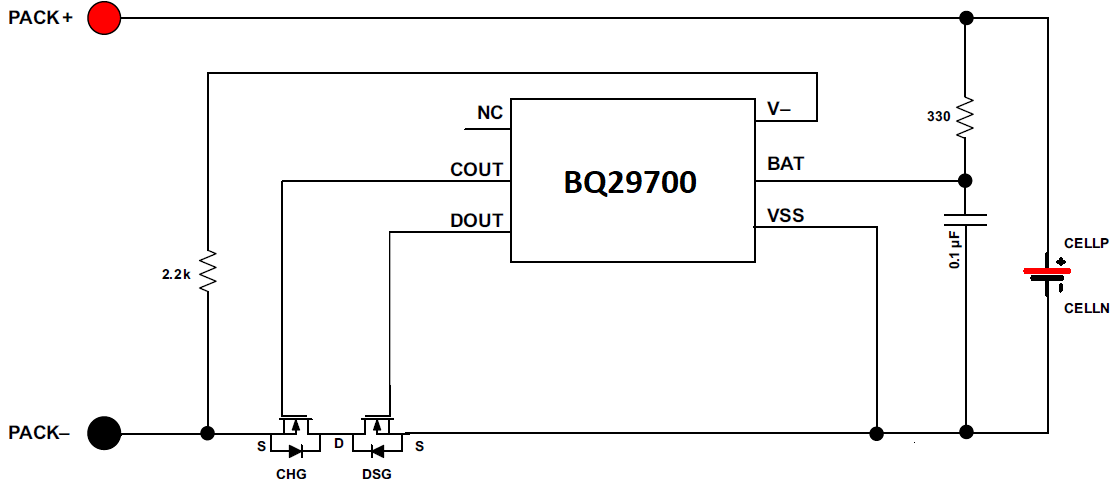
\includegraphics[width=0.9\linewidth]{bq29700_principeschema.png}
	\caption{Typical application circuit BQ29700 \cite{bib:BQ29700}}
	\label{fig:bq29700_principeschema}
\end{figure}

\subsubsection{Dimensioning}
Figure \ref{fig:bq29700_toegepast} shows the implemented BQ29700 IC in our design. An RC filter is required on the BAT-pin for noise, and enables the device to operate during sharp negative transients. The 330 $\Omega$ resistor also limits the current during a reverse connection on the system. TI recommends placing a high impedance 5 M$\Omega$ across the gate source of each external FET to deplete any charge on the gate-source capacitance. The voltage sense node $V_-$ is a sense node used for measuring several fault detection conditions, such as overcurrent charging or
overcurrent discharging configured as Vds sensing for protection. This input, in conjunction with VSS, forms the differential measurement for the stated fault detection conditions. A 2.2 k$\Omega$ resistor is connected between this input pin and Pack– terminal of the system in the application.
\\ \\
\textbf{FET Selection:} These should be MOSFETs who operate at relativly low voltages (2.8-4.2V battery cell) and that can handle a current of 1.3 A for charging (section \ref{sec:fastchargecurrent}). Due the current is measured by the voltage drop across the FETs, it's $R_{DSON}$ value is also an important value by choosing the right MOSFET. We chose FDS9926A, as it's a dual N-channel MOSFET IC. So both charge and discharge MOSFETs are integrated in one IC. Each FET's $R_{DSON}$ = 35 m$\Omega$ at Tj = 25 $^\circ$C and Vgs = 3.7 V (nominal battery voltage) \cite{bib:FDS9926A}. Because both discharge and charge overcurrent detection levels are the same (100 mV), the discharge and charge current are limited to approximately $\frac{100 mV}{2 \cdot 35m\Omega}$ = 1.43 A \cite{bib:BQ29700, bib:FDS9926A}.
\begin{figure}[H]
	\centering
	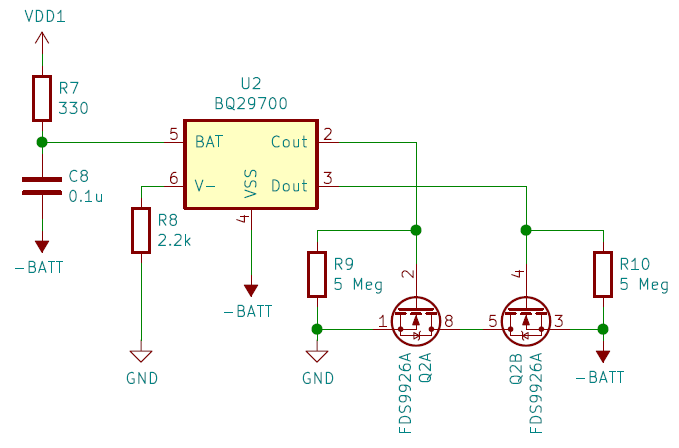
\includegraphics[width=0.9\linewidth]{bq29700_toegepast.png}
	\caption{BQ29700 applied schematic}  %% AANPASSEN!!!
	\label{fig:bq29700_toegepast}
\end{figure}


\subsection{Voltage regulator}
A few important points to consider when selecting the voltage regulator are:
\begin{enumerate}
	\item Low quiescent current $I_Q$ to reduce power losses for extended battery lifetime.
	\item Low dropout voltage\footnote{The Dropout Voltage of a regulator is the amount of voltage that a regulator needs to be fed above its rated output voltage to maintain the output voltage.} $V_{DO}$ due to the small difference between the 3.7 V nominal voltage of the battery and 3.3 V supply voltage for the ESP32 microcontroller.
	\item At least 500 mA maximum output current $I_{OUT,MAX}$ needed for ESP32 spikes \cite{bib:ESP32-SOLO-1}.
\end{enumerate}
A linear regulator is preferred over a switching regulator, because of the low dropout voltage and low quiescent current. This results in a low power dissipation in the linear regulator due Power = Voltage x Current. Another reason to chose a linear regulator over a switched regulator due the fact most inductor based switching converters struggle at very low loads \cite{LDOvsSwitch:1, LDOvsSwitch:2}

\subsubsection{Selected regulator}
As shown in figure \ref{fig:TLV75533_toegepast} we chose TLV75533 from Texas Instruments, with following parameters:
\begin{itemize}
	\item $I_Q$ = 25 $\mu$A (Typical)
	\item $V_{DO}$ = 150-238 mV (@ $I_{OUT}$ = 500 mA and $V_{OUT}$ = 3.3 V)
	\item $I_{OUT,MAX}$ = 500 mA
\end{itemize}
This device features an internal soft-start to lower inrush current, thus providing a controlled voltage to the load and minimizing the input voltage drop during start up. When shutdown, the device actively pulls down the output to quickly discharge the outputs and ensure a known start-up state. For protection reasons the TLV75533 has an integrated thermal shutdown, current limit, and undervoltage lockout (UVLO). 
\\ \\
Additionally, the TLV75533 has an enable functionality to minimize standby power. Unfortunately we can't use this function because the LDO supplies the microcontroller (these control signals to drive the enable pin should originate from the microcontroller). Therefor the enable pin is connected to the input pin to enable when an input voltage is supplied. 
\\ \\
The TLV75533 requires an output capacitance of 0.47-200 $\mu$F for stability. Use X5R- and X7R-type ceramic capacitors because these capacitors have minimal variation in capacitance value and equivalent series resistance (ESR) over temperature. Place a 1 $\mu$F or greater capacitor on the input pin of the LDO. Some input supplies have a high impedance. Placing a capacitor on the input supply reduces the input impedance \cite{bib:TLV755P}.
\begin{figure}[H]
	\centering
	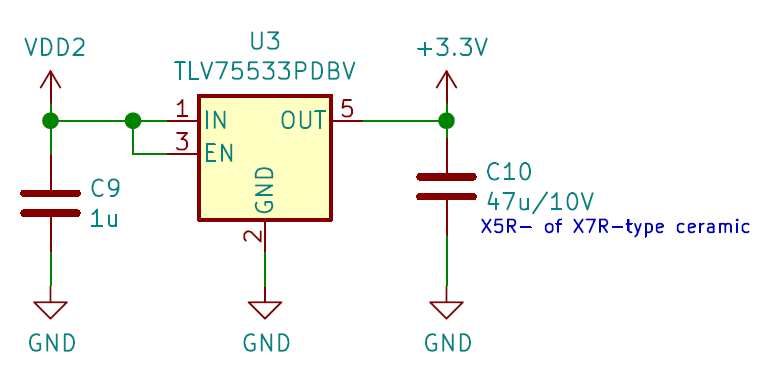
\includegraphics[width=0.9\linewidth]{TLV75533_toegepast.png}
	\caption{TLV75533 applied schematic}
	\label{fig:TLV75533_toegepast}
\end{figure}

\subsection{Load switches}
To reduce power even further you can disable the sensors by shutting off their supply voltage if they're not needed. This can be done by load switches or relays. A load switch is a small electronic switch used to configure and manage power distribution. You can make a load switch with discrete components, but there are significant advantages to using a fully integrated IC load switch \cite{loadSwitch}:
\begin{enumerate}
	\item \textbf{Saves space:} A key advantage of the integrated device over discrete load switches is the small footprint. 
	\item \textbf{Simpler design:} No discrete design time is required. Just buy the integrated chip and design it in to get all benefits and features.
\end{enumerate}
Load witches also has several advantages over relays \cite{loadSwitch}:
\begin{enumerate}
	\item \textbf{Quick output discharge:} An internal resistance in the form of a conducting MOSFET is connected across the load. It serves to discharge to the output capacitor quickly when the enable input goes low.
	\item \textbf{Reverse-current blocking:} Some IC load switches implement a feature that blocks any reverse current. When the enable input goes low to turn off the switch, the reverse current block circuit is enabled thereby reducing any potential reverse current from output back to input to a very low level.
	\item \textbf{Saves power:} Using load switches to manage the power output of the supply minimizes power consumption, saves energy, and provides for longer battery life in portable applications. In its off state, the IC draws minimal quiescent current.
	\item \textbf{Manages inrush current:} This feature prevents input voltage droop that may transpire when the switch is first turned on. This is the result of a high inrush current that occurs when charging the output capacitor. Most load switches provide a controlled ramp up of the output voltage as it charges the output capacitor.
	\item \textbf{Implements sequencing:} Load switches let you implement the sequencing of loads during a turn-on or turn-off operation. Some designs with processors, FPGAs, and other chips require that different supply voltages be applied or disconnected in a specific order. Multiple load switches for each supply that are operated by the related embedded controller for timing meet this need. Certain load switches also feature an output signal that indicates when the output is fully turned on. This signal can be used in sequencing operations with other load switches in the system.
\end{enumerate}

\subsubsection{Selected load switches}
The TPS22919 device is a small, single channel load switch with controlled slew rate. The device contains an N-channel MOSFET that can operate over an input voltage range of 1.6 V to 5.5 V and can support a maximum continuous current of 1.5 A. A few important specifications are \cite{bib:TPS22919}:
\begin{itemize}
	\item Input operating voltage range $V_{IN}$: 1.6 V to 5.5 V
	\item Maximum output current $I_{OUT,MAX}$ = 1.5 A
	\item Low power consumption:
	\begin{itemize}
		\item ON-state $I_Q$ = 8 $\mu$A (typical)
		\item OFF-state $I_{SD}$ = 2 nA (typical)
	\end{itemize}
	\item On-Resistance $R_{ON}$: 89 m$\Omega$ (typical) @ $V_{IN}$ = 5 V
\end{itemize}
The switch ON state is controlled by a digital input that is capable of interfacing directly with low-voltage control signals. When power is first applied, a Smart Pull Down is used to keep the ON pin from floating until system sequencing is complete. Once the pin is deliberately driven High ($> V_{IH}$), the Smart Pull Down will be disconnected to prevent unnecessary power loss. The TPS22919 load switch is also self-protected, meaning that it will protect itself from short circuit events on the output of the device. It also has thermal shutdown to prevent any damage from overheating.
\\ \\
Figure \ref{fig:TPS22919_toegepast} shows the application of TPS22919 for our 3 sensors. The resistor between VOUT and QOD pin is a quick discharge resistor to discharge the output capacitor when the enable pin goes low. For both in- and output capacitors, and the resistor, we used the recommended value as given in the datasheet \cite{bib:TPS22919}.
\begin{figure}[H]
	\centering
	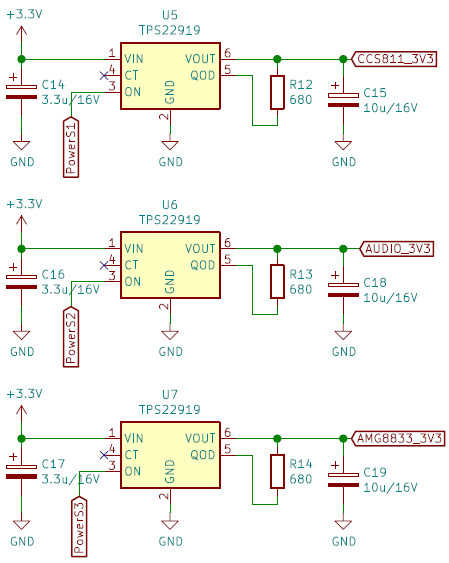
\includegraphics[width=0.8\linewidth]{TPS22919_toegepast.png}
	\caption{TPS22919 applied schematic}
	\label{fig:TPS22919_toegepast}
\end{figure}


\section{Microcontroller}
\begin{figure}[H]
	\centering
	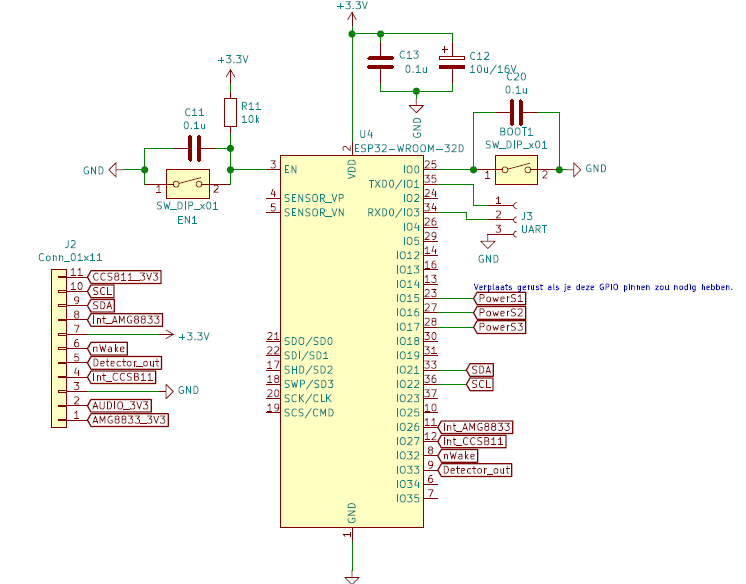
\includegraphics[width=1.0\linewidth]{ESP32_toegepast.png}
	\caption{ESP32 applied schematic}
	\label{fig:ESP32_toegepast}
\end{figure}

\section{Sensorboard}

% ============ Geofrey wil zien dat we hebben nagedacht over de dimensionering van de componenten !!! ============


\section{Wireless connectivity}
\subsection{Wi-Fi connection}
In order to transmit the sensor data to the server, the Wi-Fi connectivity of the ESP32 is used. The transmission is provided by a TCP connection that is established between the ESP32 and the python server. At the initialisation of the python server, a socket is opened, this socket is used to receive the data. In this manner, the server is always listening on the socket, until a message is received. The ESP32 sends the data in the following order: pixeldata (64 floats), temperature (1 float), audio level (1 float), $CO_2$-level (1 unint16) and TVOC-level (1 unint64). The received data is processed by order to determine which data is represented by the received values. The data is parsed into different variable, these variables are then used to update the values in the database. 

\subsection{Power consumption}
To determine the power that is consumed when the sensor data is transmitted once, a measurement is performed. The current consumption is measured, the result is displayed in figure~\ref{fig:wifi_pwr}.
\begin{figure}[H]
	\centering
	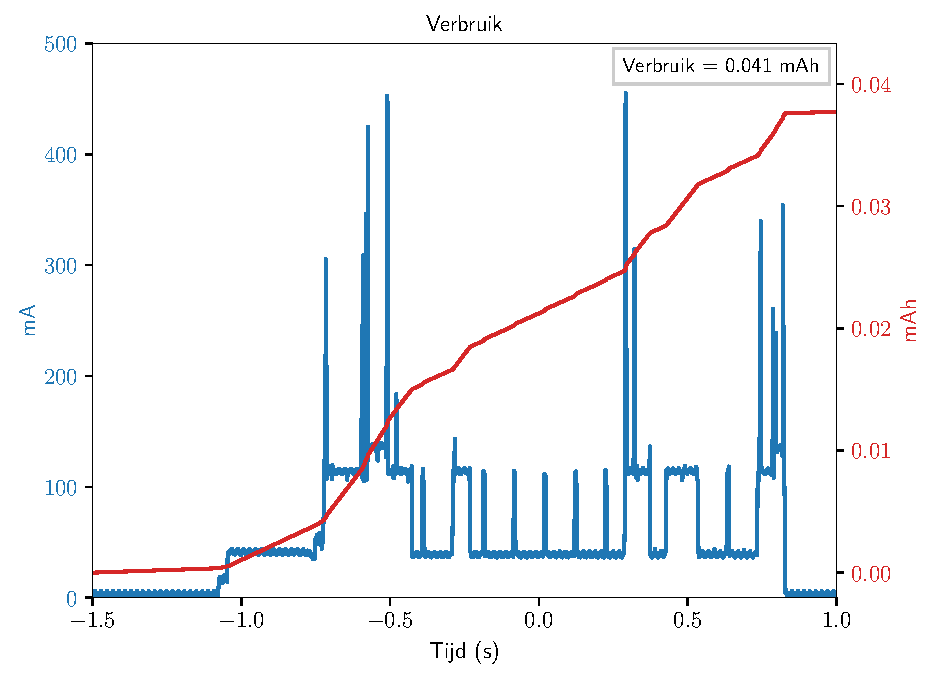
\includegraphics[width=1.0\linewidth]{wifi_pwr.pdf}
	\caption{Power consumption of one Wi-Fi transmission}
	\label{fig:wifi_pwr}
\end{figure}
In order to interpret the current consumption, the used capacity is displayed in [mAh]. This results in 0.041 mAh of capacity that is used in order to transmit the sensor data once. With this knowledge, we can calculate the amount of Wi-Fi transmissions that are possible with the 6400 mAh battery:

\begin{gather*}
	\frac{6400}{0.041} \approx 156097
\end{gather*}

156097 transmissions are possible, if there are 6 transmissions per hour and the system is active for 7 hours a day, this leads to a battery life off 3716 days.  However, this calculation only accounts for the Wi-Fi transmission other power consumption such as stand-by power, CPU power and sensor power are not accounted for in the calculation. 

\section{Software design}
\textbf{todo}
\begin{figure}[H]
	\centering
	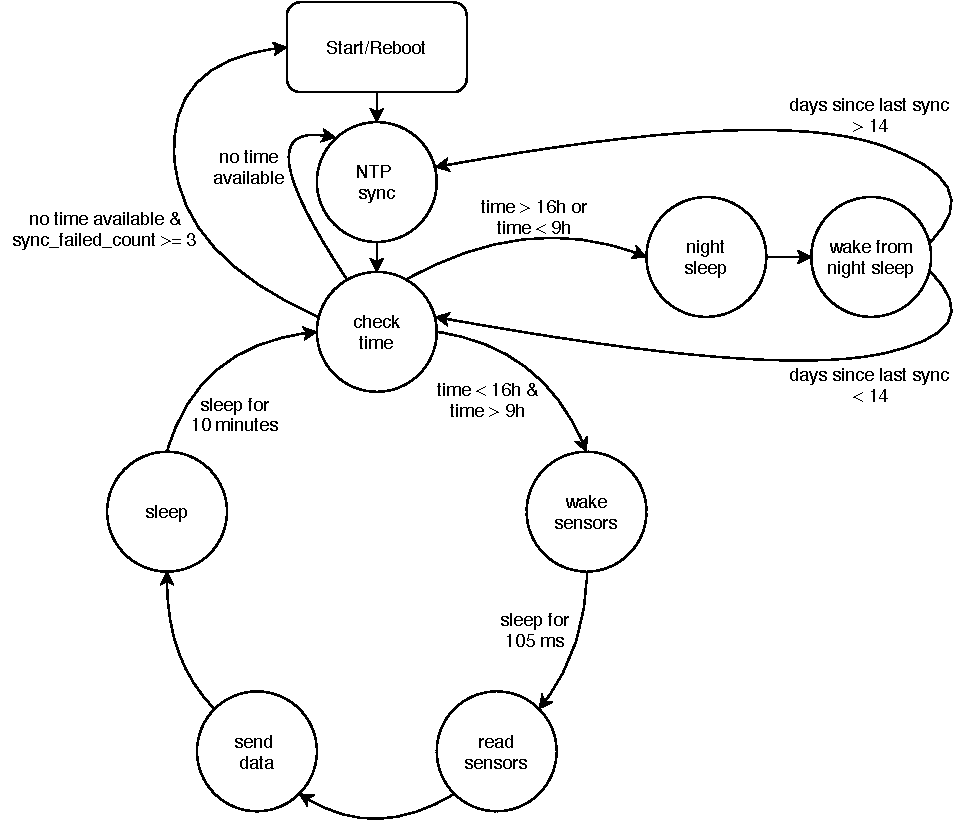
\includegraphics[width=0.8\linewidth]{statendiagram.pdf}
	\caption{State diagram}
	\label{fig:statediagram}
\end{figure}

\section{Autonomy}
Calculations for lifetime.

\section{Website}

\section{Financial estimate}
Kostprijs van het project opstellen.

\section{Validation and measurements}
Hier moeten we aantonen of dat alles werkt. Of eventuele fouten verklaren.

% bibliografie toevoegen
\newpage
\bibliography{bibliography}	

%----------------------------------------------------------------------------------------
%	Bijlagen
%----------------------------------------------------------------------------------------
\newpage
\appendix
\section{MainPCB schematic}\label{app:mainpcb_schematic}
%\begin{figure}[H]
%	\centering
%	\includegraphics[width=1\linewidth]{MainPCB_schematic.pdf}
%\end{figure}
\includepdf[pages=-]{fig/MainPCB_schematic.pdf}

\newpage

\end{document}